% This file was created by tikzplotlib v0.8.5.
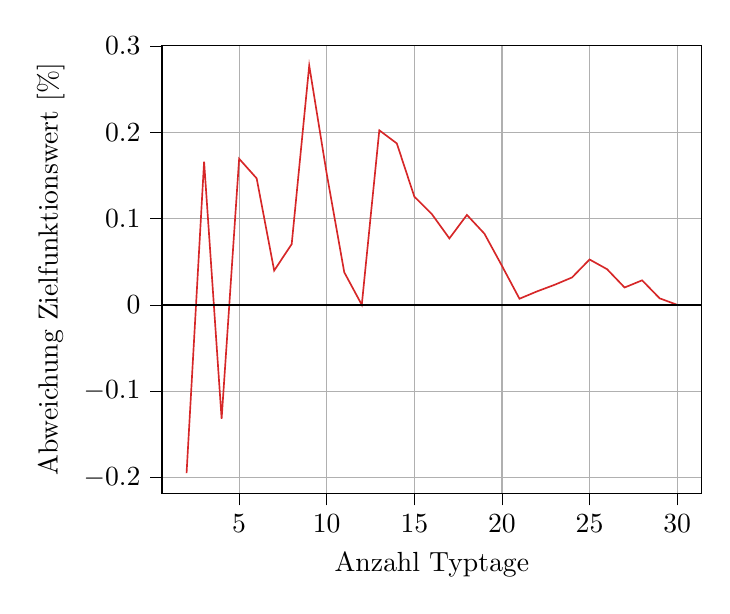
\begin{tikzpicture}

\definecolor{color0}{rgb}{0.83921568627451,0.152941176470588,0.156862745098039}

\begin{axis}[
tick align=outside,
tick pos=left,
x grid style={white!69.01960784313725!black},
xlabel={Anzahl Typtage},
xmajorgrids,
xmin=0.6, xmax=31.4,
xtick style={color=black},
y grid style={white!69.01960784313725!black},
ylabel={Abweichung Zielfunktionswert [\%]},
ymajorgrids,
ymin=-0.218516765308908, ymax=0.300789621945624,
ytick style={color=black}
]
\addplot [semithick, color0]
table {%
1 nan
2 -0.194911929524611
3 0.165870770127585
4 -0.131980837233174
5 0.169187504389135
6 0.146461947714772
7 0.0396677510360999
8 0.0703365206156036
9 0.277184786161327
10 0.151611426483501
11 0.037639376497256
12 -1.61044965338525e-05
13 0.202111695507796
14 0.186923835235688
15 0.125238333348294
16 0.105031678336706
17 0.0768939547944142
18 0.104112666001718
19 0.0823702756403385
20 0.0451398477517859
21 0.00701918441549378
22 0.0155131183004634
23 0.0231120645911755
24 0.0316738485680989
25 0.0524943225049515
26 0.0412396555010583
27 0.0200239613787772
28 0.0283602824042269
29 0.0074986231975504
30 0
};
\addplot [thick, black]
table {%
0.6 0
31.4 0
};
\end{axis}

\end{tikzpicture}
